\documentclass[fleqn]{article}
\usepackage{fontspec}
\usepackage{polyglossia}
\setdefaultlanguage{english}
\usepackage[a4paper,margin=2cm]{geometry}

\usepackage{amsmath}
\usepackage{amssymb}
\usepackage{array}
\usepackage{auto-pst-pdf}
\usepackage{booktabs}
\usepackage{cite}
\usepackage{graphicx}
\usepackage{lmodern}
\usepackage{marvosym}
\usepackage{mathrsfs}
\usepackage{minted}
\usepackage{multicol}
\usepackage{multirow}
\usepackage{paralist}
\usepackage{schemabloc}
\usepackage{siunitx}
\usepackage{soul}
\usepackage{tikz}
\usepackage[european,cuteinductors,siunitx]{circuitikz}
\usepackage{url,hyperref}
\usepackage{verbatim}
\usepackage{xunicode,xltxtra}

\title{
\includegraphics{../../images/inp-enseeiht} \\ ~ \\ ~ \\ ~ \\ ~ \\ Phase-shift  laser  rangefinder – AMS VHDL}
\author{Meszaros Csongor \& Guilhem Saurel}
\date{\oldstylenums{\today}}

\begin{document}

\begin{titlepage}
    \setcounter{page}{0}
    \maketitle
    \vfill
    \tableofcontents
    \thispagestyle{empty}
\end{titlepage}

\section{Introduction}

Laser range finders are widely used in the fields like spaceflight, robot vision, mapping, and mechanical manufacturing for their merits of being non-contact, high precision and low cost. The three major techniques used for laser range finder are time of flight (TOF), frequency modulation continuous wave (FMCW) and phase-shift measurement. In these methods, phase-shift measurement can achieve higher resolution in a long distance.

In this paper a phase-shift laser ranging method is modeled using AMS-VHDL hardware description language.

\section{Principle of phase-shift laser range finder}

As shown in figure 1, a laser beam with intensity modulated at a  particular frequency is emitted to the target, and reflected back. And phase-shift is produced in the received beam due to the time delay between the emitted point and the target.

\begin{figure}[h]
    \begin{center}
        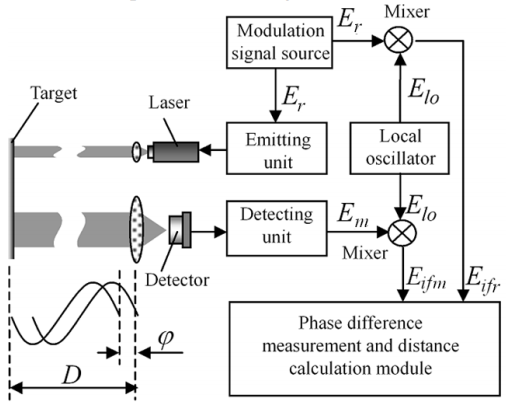
\includegraphics[width=10cm]{block.png}
    \end{center}
    \caption{Block diagram of phase-shift laser range finder}
\end{figure}

Distance D can be obtained by measuring the phase-shift, and expressed as in the equation:

\begin{eqnarray}
    D&=&\cfrac{c}{2f}\cfrac{\Delta\varphi}{2\pi}
\end{eqnarray}

Where $c$ is the velocity, $f$ is the modulation frequency, and $\Delta\varphi$ is the phase-shift between measured signal and reference signal. When modulation frequency $f$ is determined, the non-ambiguity range fors a laser rangefinder is

\begin{eqnarray}
    D_{nar}&=&\cfrac{c}{2f}
\end{eqnarray}

and the resolution of distance measurement can be expressed as

\begin{eqnarray}
    \delta D_{min}&=&\cfrac{c}{2f}\cfrac{\delta\varphi_{min}}{2\pi}
\end{eqnarray}

Equation (3) indicates that distance measurement resolution is $\delta D_{min}$ is directly determined by the phase-shift resolution $\delta\varphi_{min}$.

~

Equation (1) shows that the phase-shift $\Delta\varphi$ between the measurement signal and reference signal must be measured accurately to obtain a precise distance measurement.

~

The laser diode is driven with a sinus modulated signal generated by the RF oscillator at 20 MHz – to achieve accurate measurement. The emitted beam is reflected by the Lambertian target and the reflected laser beam is converted to the electrical signal using a photo-diode. It is difficult to deal with an RF signals, to design electronic circuits in the low-frequency domain is much easier. Hence of that, it is necessary to demodulate the RF signal. To accomplish a demodulation, the  RF signal from the photo-diode is multiplied with the frequency of the local oscillator – 19.5 MHz. This way the frequency is reduced to around 5 kHz, what is in a low-frequency range, easy to design electronic environment for signal processing.

~

 The demodulating is achieved in a quite unpretentious way. The RF signal is simply multiplied by the signal of the local oscillator (the mathematical calculation is shown below) . The mixer produces  new signals at the sum $f_1 + f_2$ and difference $f_1 - f_2$ of the original frequencies. Which implies that a band-pass filter is needed to filter out all unwanted components. The center frequency of the band-pass filter is 5 kHz.

~

There are many different ways how to achieve a last step – the comparison. One method, which could be named digital way as well, is to use low-pass filters and zero-crossing comparators to get a phase-difference. Zero-cross comparators are used to convert sine wave signals into square waves. Then the task to measure phase-shift is also converted to measure the phase difference between two square waves. This method is illustrated on the figure 2.

\begin{figure}[h]
    \begin{center}
        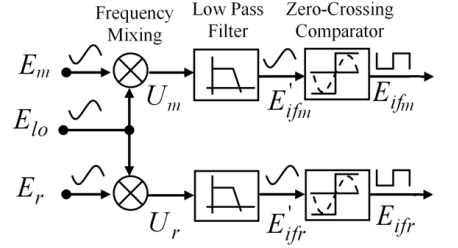
\includegraphics[width=10cm]{fin.png}
    \end{center}
    \caption{Heterodyne processing and digital conversion}
\end{figure}

\begin{figure}[h]
    \begin{center}
        %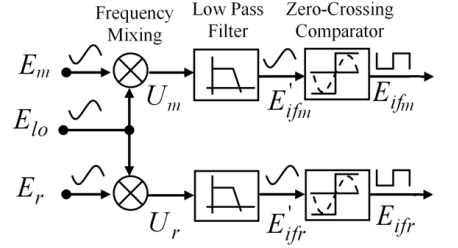
\includegraphics[width=10cm]{fin.png} TODO
    \end{center}
    \caption{Phase shift measurement using PLL}
\end{figure}

In this particular case the so-called analog principle is used to get a phase-shift between the two signals – figure 3. The difference toward to above mentioned technique is using the PLL (Phase Locked Loop).

~

On one input of the PLL the reflected 5 kHz signal is connected. The second input of the PLL is feed by the original 5 kHz signal of the local oscillator. The only difference between those two signals is the phase difference, what is utilized to calculate the distance from the target.

~

This paper contains the way where the PLL is modeled using an ideal operational amplifier and 4 serial connected first order passive low-pass filters. The operational amplifier has very high gain (A = 100 000) and infinite input resistance.

\section{Mathematical demonstration}
\subsection{Emitted signal}
\begin{eqnarray}
v_{LD} &=& V_{LD} \cdot \cos\left(2\pi f_{RF}t+\theta_1\right) \nonumber
\end{eqnarray}
\subsection{Reflected signal (photo-diode)}
\begin{eqnarray}
v_{PD} &=& V_{PD} \cdot \cos\left(2\pi f_{RF}t+\varphi(D)+\theta_0\right) \nonumber
\end{eqnarray}

$\varphi(D)$ - phase-shift: function of the measured distance

\subsection{Local oscillator}
\begin{eqnarray}
v_{LO} &=& V_{LO} \cdot \cos\left(2\pi f_{LO}t+\theta_2\right) \nonumber
\end{eqnarray}
\subsection{Reference signal}
\begin{eqnarray}
v_{ref}(t) &=& v_{LD}(t)\cdot v_{LO}(t) = V_{LD}\cdot\cos\left(2\pi f_{RF}t + \theta_1\right)\times V_{LO}\cdot\cos\left(2\pi f_{LO}t + \theta_2\right) \nonumber
\end{eqnarray}
using a low-pass filter the component with $\left(f_{RF}+f_{LO}\right)$ is eliminated
\begin{eqnarray}
v_{ref}(t) &=& V_0\cdot\cos\left(2\pi|f_{RF}-f_{LO}|t+\theta_1-\theta_2\right) \nonumber
\end{eqnarray}
\subsection{Measured signal}
\begin{eqnarray}
v_{meas}(t)&=&v_{PD}(t)\cdot v_{LO}(t) =V_{PD} \cdot \cos\left(2\pi f_{RF}t+\varphi(D)+\theta_0\right)\cdot V_{LO} \cdot \cos\left(2\pi f_{LO}t+\theta_2\right) \nonumber \\
v_{meas}(t)&=&V_S\cdot\cos\left(2\pi|f_{RF}-f_{LO}|t+\varphi(D)+\theta_0-\theta_2\right) \nonumber
\end{eqnarray}


According to the equation (2) the distance limitation can be calculated. Theoretically it is 7.5 meter, however, it can be seen on the simulation results that this value is around 2.5 meter. Because the $\Delta V$ on the output above 2.5 meter is around a few $\mu V$ – so it is very hard to make a distinction between that small variations of voltage levels.

\section{Architecture and Implementation overview}

%TODO

\section{Conclusion}

The described system in this paper is a model what can be used for range measuring. The system is modelled in AMS-VHDL hardware description language. The model demonstrates how to use a laser to calculate the distance from the target based on a phase-shift measurement.

~

As the simulation results demonstrate the model behaves according to the expectations. How the distance $D$ is changing, the phase-difference on the output between the two signals is changing.

~

As the system is constructed mostly with ideal elements with ideal characteristics, this project has an educational purpose to show the basic functionality. To make this model usable it is necessary to replace the ideal components by real ones.








\end{document}
